\documentclass[11pt]{beamer}  %% versione proiettore
%%\documentclass[11pt,handout]{beamer} %% versione stampa
\usepackage{lucidiJb-2ed}

\usepackage{relsize}

\mode<article>
{
  \usepackage{fullpage}
  \usepackage{hyperref}
}

\mode<presentation>
{
  \setbeamertemplate{background canvas}[vertical shading][bottom=red!10,top=blue!10]
  \usetheme{Ethereum}
  \usefonttheme[onlysmall]{structurebold}
}

\subtitle{Learning Ethereum}
\title{Smart Contract Security}
\institute{Universit\`a di Verona, Italy}
\date{January 2020}

\setbeamercovered{invisible}

\def\codesize{\smaller}
\def\<#1>{\codeid{#1}}
\newcommand{\codeid}[1]{\ifmmode{\mbox{\codesize\ttfamily{#1}}}\else{\codesize\ttfamily #1}\fi}

\begin{document}

\begin{frame}
  \titlepage
\end{frame}

\begin{frame}\frametitle{Security best practice}

  \begin{itemize}
  \item Minimalism: the simpler, the better
  \item Code reuse: DRY, use well-known libraries
  \item Study: be aware of well-known issues and solutions
  \item Readability: simpler audit
  \item Test: try corner cases
  \item Analysis: static or dynamic, still in infancy
  \end{itemize}

  \bigskip

  \begin{redbox}{}
    Considering the importance of security for smart contracts,
    it is questionable why the invented Solidity (hard, new, convoluted
    semantics) for writing such delicate pieces of software.
  \end{redbox}

  \bigskip

  \begin{center}
    Remember the DAO
  \end{center}
  
\end{frame}

\begin{frame}\frametitle{Issue \#1: Reentrancy}

  \begin{redbox}{}
    Our contract calls an unknown contract. The latter, unexpectedly, calls
    back into our contract again. Particularly dangerous if this cycle
    is triggered by a call sending ETH, that would be repeated as many
    times as the unknown contract decides.
  \end{redbox}

  \bigskip

  \begin{greenbox}{Three ways of sending ETH}
    \begin{description}
    \item[\<c.send(amount)>] forwards $2300$ units of gas,
      \alert{currently not enough for reentrancy}; possibly
      deprecated in the future
    \item[\<c.transfer(amount)>] forwards $2300$ units of gas,
      \alert{currently not enough for reentrancy}; possibly
      deprecated in the future
    \item[\<c.call.value(amount)()>] forwards all remaining units of gas,
      typically \alert{enough for reentrancy}; programmers like it since
      it allows one to activate the complex fallback function of any
      contract, not just the default fallback function
    \end{description}
  \end{greenbox}
  
\end{frame}

\begin{frame}\frametitle{Reentrancy: prevention}

  \begin{greenbox}{Use the checks/effects/interactions pattern}
    \begin{center}
      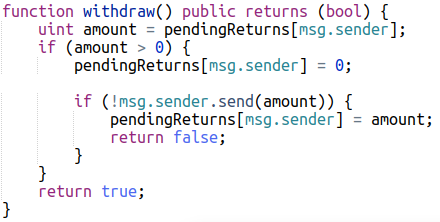
\includegraphics[scale=0.4,clip=false]{pictures/simple-auction-withdraw-only.png}
    \end{center}
  \end{greenbox}

  \medskip

  \begin{greenbox}{Use a mutex to ban reentrancy}
    \begin{center}
      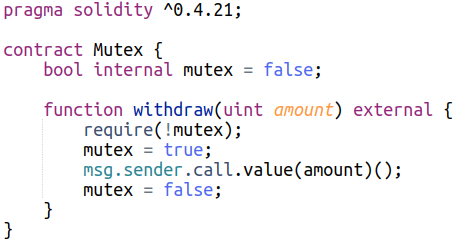
\includegraphics[scale=0.35,clip=false]{pictures/mutex.png}
    \end{center}
  \end{greenbox}
  
\end{frame}

\begin{frame}\frametitle{Issue \#2: Arithmetic over/underflows}

  \begin{redbox}{}
    An operation tries to compute a fixed-size value that is outside the
    bounds for its type.
  \end{redbox}

  \bigskip

  \begin{greenbox}{What if an account with $0$ balance tries to send $1$ ETH to another account?}
    \begin{center}
      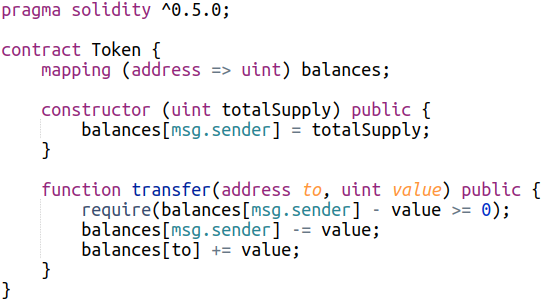
\includegraphics[scale=0.5,clip=false]{pictures/under-overflow.png}
    \end{center}
  \end{greenbox}
  
\end{frame}

\begin{frame}\frametitle{Over/underflows: prevention}

  \begin{greenbox}{Test numerical operations}
    \begin{center}
      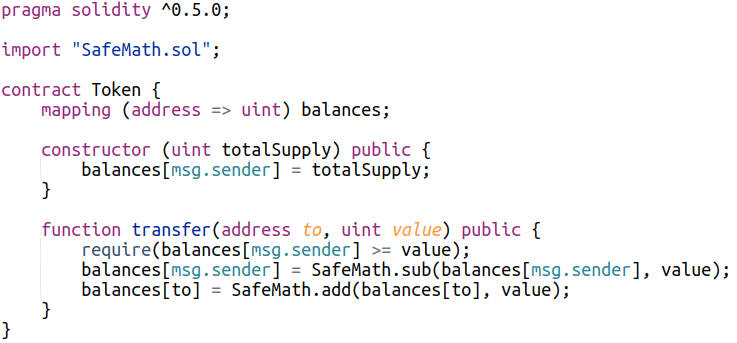
\includegraphics[scale=0.5,clip=false]{pictures/under-overflow-fixed.png}
    \end{center}
  \end{greenbox}
    
\end{frame}

\begin{frame}\frametitle{Over/underflows: prevention}

  \begin{greenbox}{Replace numerical operations with a library for safe arithmetic}
    \begin{center}
      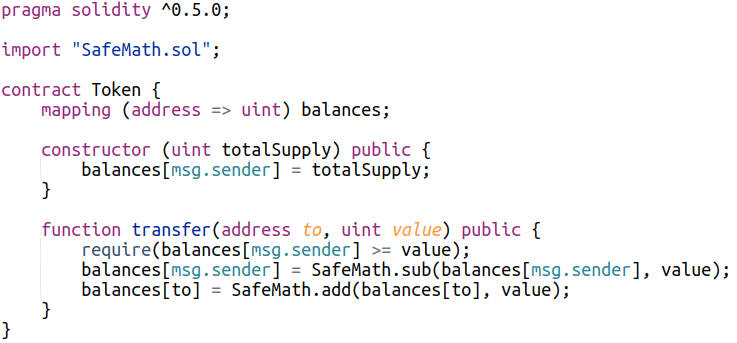
\includegraphics[scale=0.45,clip=false]{pictures/under-overflow-fixed.png}
    \end{center}
  \end{greenbox}
    
\end{frame}

\begin{frame}\frametitle{Over/underflows: prevention}

  \begin{greenbox}{A library for safe arithmetic}
    \begin{center}
      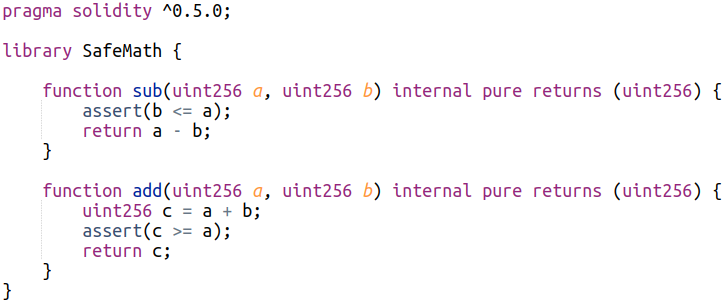
\includegraphics[scale=0.45,clip=false]{pictures/safe-math.png}
    \end{center}
  \end{greenbox}

  \medskip

  \begin{center}
    \url{https://docs.openzeppelin.com/contracts/2.x/api/math}
  \end{center}
  
\end{frame}

\begin{frame}\frametitle{Issue \#3: Unexpected ether}

  \begin{redbox}{}
    Code correctness depends on invariants about \<this.balance>,
    that actually do not hold.
  \end{redbox}

  \bigskip

  \begin{greenbox}{This code assumes \<this.balance \% 0.5 ether == 0>. But this is false
      since it is possible to send $0.1$ ether to this contract\ldots}
    \begin{center}
      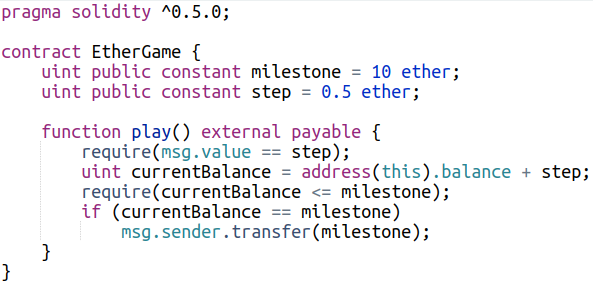
\includegraphics[scale=0.5,clip=false]{pictures/unexpected-ether.png}
    \end{center}
  \end{greenbox}

\end{frame}

\begin{frame}\frametitle{Issue \# 3: Unexpected ether}

  \begin{redbox}{}
    It is possible to send ether to a contract, without calling any \<payable> function
    nor its fallback function (if any)!
  \end{redbox}

  \bigskip

  \begin{greenbox}{How?}
    \begin{itemize}
    \item write a suicidal contract that executes \<selfdestruct(beneficiary)>
      and forwards its balance to \<beneficiary>: it does not even call
      the fallback function of \<beneficiary>!
    \item let ether be there from the very beginning, by sending ether
      to the address of the contract before its same creation!
      Remember that the address of a contract is computed deterministically
      from the address of the creator and from its current nonce
    \end{itemize}
  \end{greenbox}
  
\end{frame}

\begin{frame}\frametitle{Unexpected ether: prevention}

  \begin{greenbox}{Do not rely on \<this.balance>}
    Use your own counter instead.
  \end{greenbox}

  \bigskip

  \begin{center}
    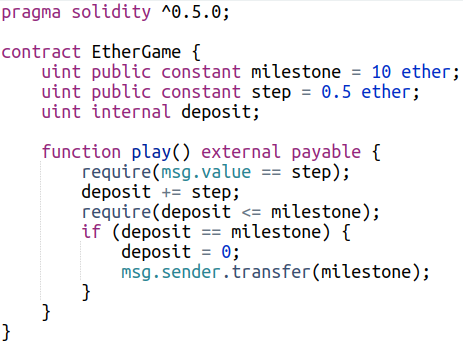
\includegraphics[scale=0.5,clip=false]{pictures/unexpected-ether-fixed.png}
  \end{center}  

\end{frame}

\end{document}
